% Created 2018-08-17 Fri 21:49
% Intended LaTeX compiler: pdflatex
\documentclass[xcolor=svgnames,t,10pt,allowframebreaks]{beamer}
\usepackage[utf8]{inputenc}
\usepackage[T1]{fontenc}
\usepackage{graphicx}
\usepackage{grffile}
\usepackage{longtable}
\usepackage{wrapfig}
\usepackage{rotating}
\usepackage[normalem]{ulem}
\usepackage{amsmath}
\usepackage{textcomp}
\usepackage{amssymb}
\usepackage{capt-of}
\usepackage{hyperref}
\usepackage{minted}
\newsavebox{\mybox}
\usefonttheme[onlymath]{serif}
\usetheme[sectionpage=progressbar,subsectionpage=progressbar,numbering=counter,progressbar=foot,block=transparent]{metropolis}
\author{William Oquendo, woquendo@gmail.com}
\date{}
\title{Linear Systems: Matrices, eigen-values, \ldots{}}
\subtitle{Herramientas de Modelación - Maestría en Gestión y Diseño de Procesos}
\AtBeginSection[]{
\begin{frame}<beamer>\frametitle{Topic}\tableofcontents[currentsection,currentsubsection]\end{frame}
}
\hypersetup{colorlinks=true, linkcolor=blue}
\hypersetup{
 pdfauthor={William Oquendo, woquendo@gmail.com},
 pdftitle={Linear Systems: Matrices, eigen-values, \ldots{}},
 pdfkeywords={},
 pdfsubject={},
 pdfcreator={Emacs 25.3.1 (Org mode 9.1.4)}, 
 pdflang={English}}
\begin{document}

\maketitle
\begin{frame}{Outline}
\tableofcontents
\end{frame}


\section{Linear Systems and Matrices}
\label{sec:org8240dae}
\begin{frame}[label={sec:org9eec588}]{Example : Bungee-jumping family plan \cite{chapra2012AppliedNumericalMethods}}
\vfill
\begin{center}
\begin{figure}[H]

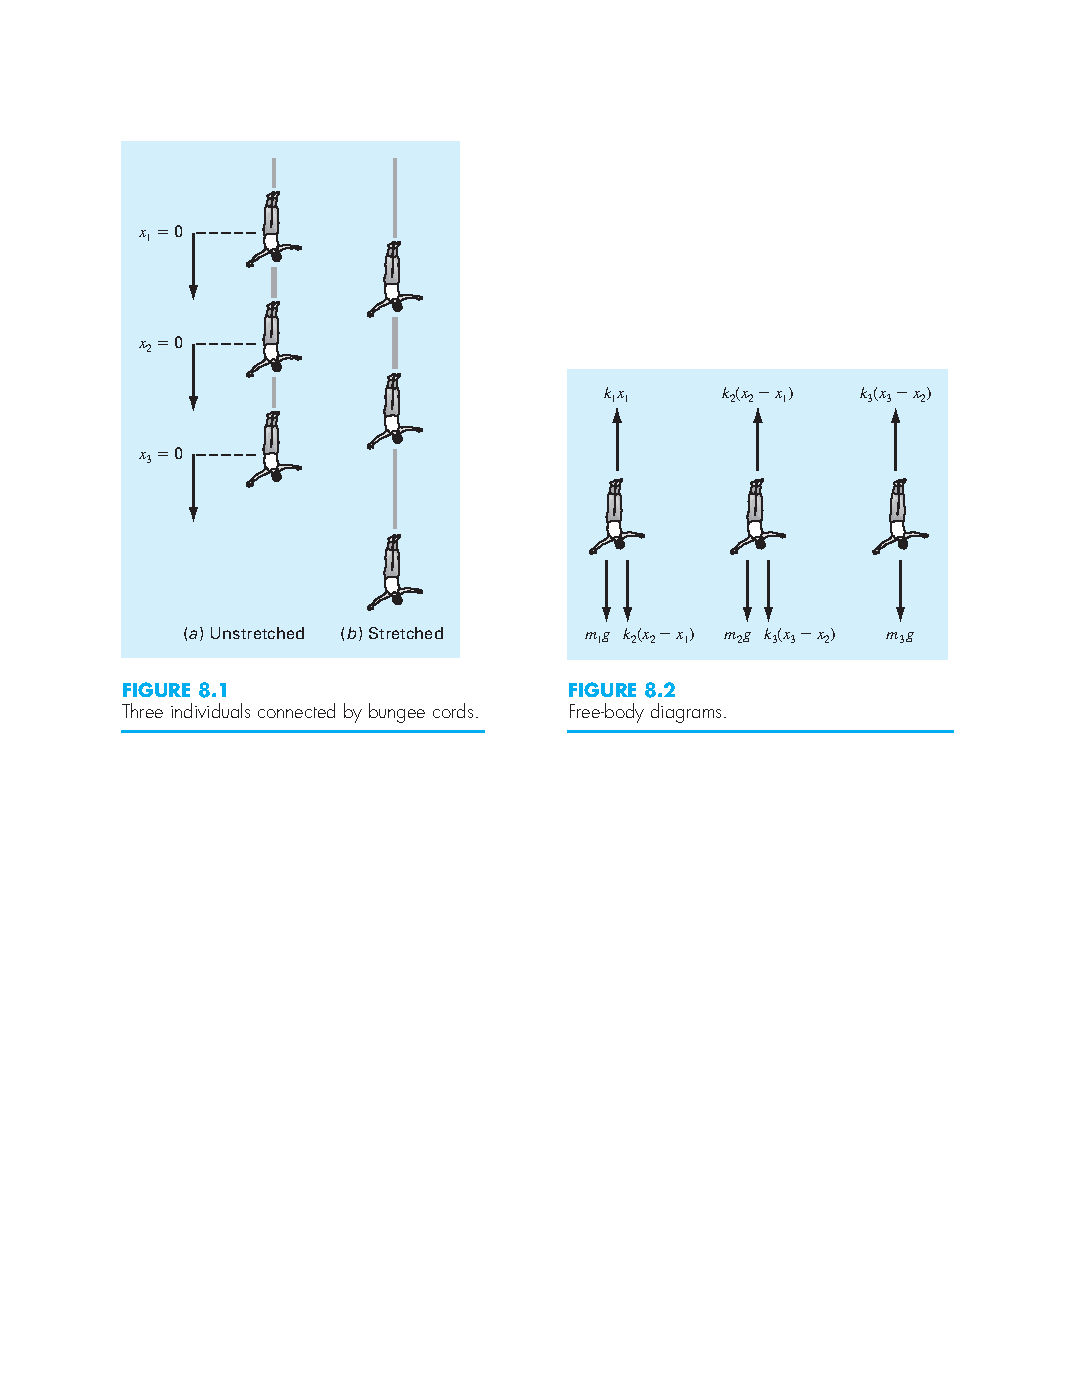
\includegraphics[width=1.0\textwidth]{fig/bungee-family-01.pdf}
\end{figure}
\end{center}
\vfill
\end{frame}

\begin{frame}[label={sec:orgc07093e}]{Example : System of equations}
\vfill
\begin{center}
\only<1->{
The second Newton law produces: 
\begin{figure}[H]

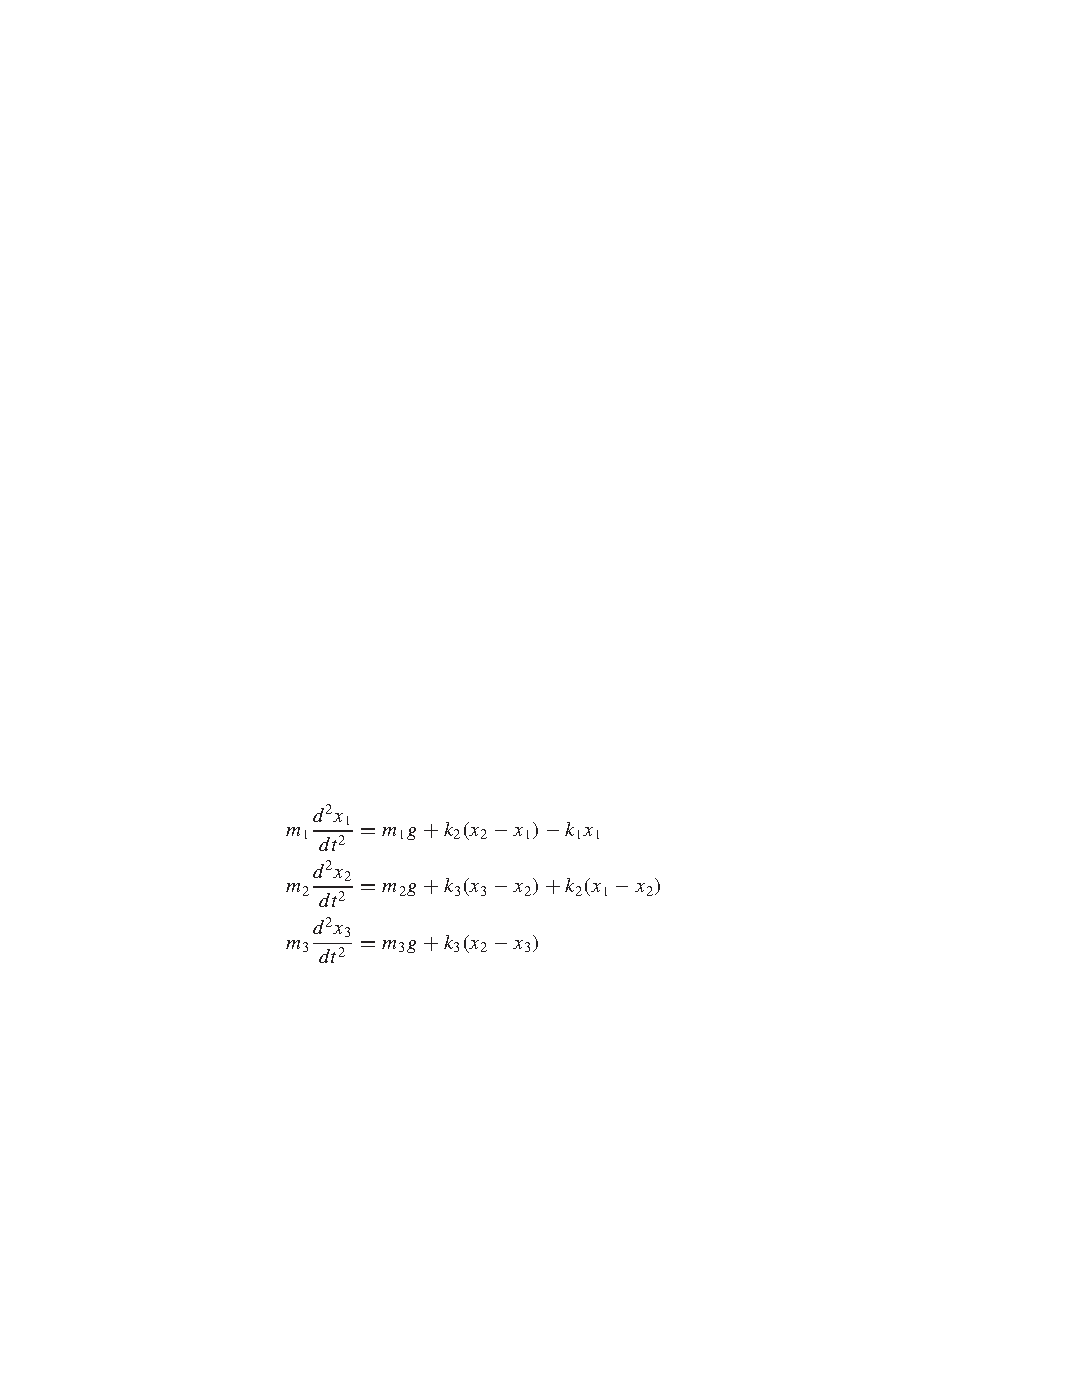
\includegraphics[width=0.5\textwidth]{fig/bungee-family-equ-00.pdf}
\end{figure}
\end{center}
\vfill
\begin{center}
}\only<2->{
And for a system in equilibrium, we get:
\begin{figure}[H]


\includegraphics[width=0.7\textwidth]{fig/bungee-family-equ.pdf}
\end{figure}
}
\end{center}
\vfill
\end{frame}

\begin{frame}[label={sec:orga29f205}]{A matrix}
\begin{figure}[H]

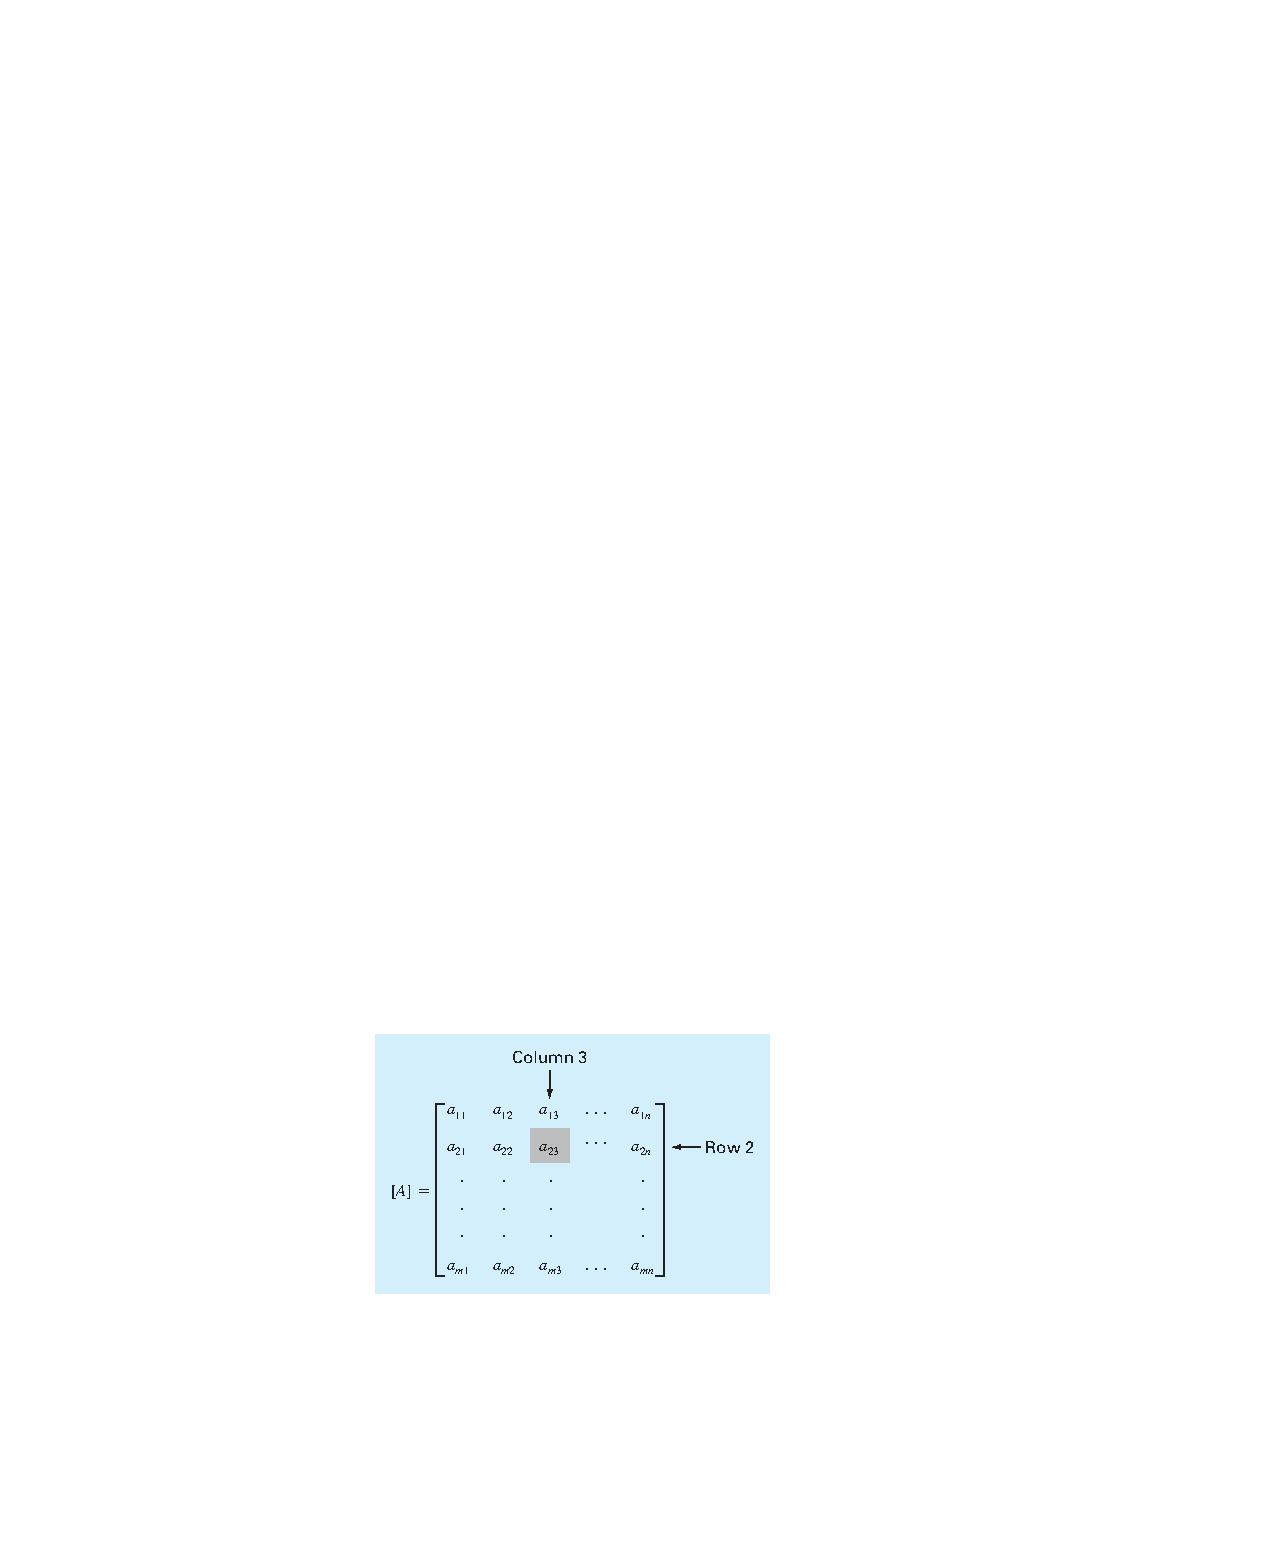
\includegraphics[width=0.9\textwidth]{fig/matrix-base.pdf}
\end{figure}
\end{frame}

\begin{frame}[label={sec:org2d257f2}]{Special cases}
\begin{columns}
\begin{column}{0.45\columnwidth}
\begin{block}{}
\begin{itemize}
\item <1-> A symmetric matrix :\\
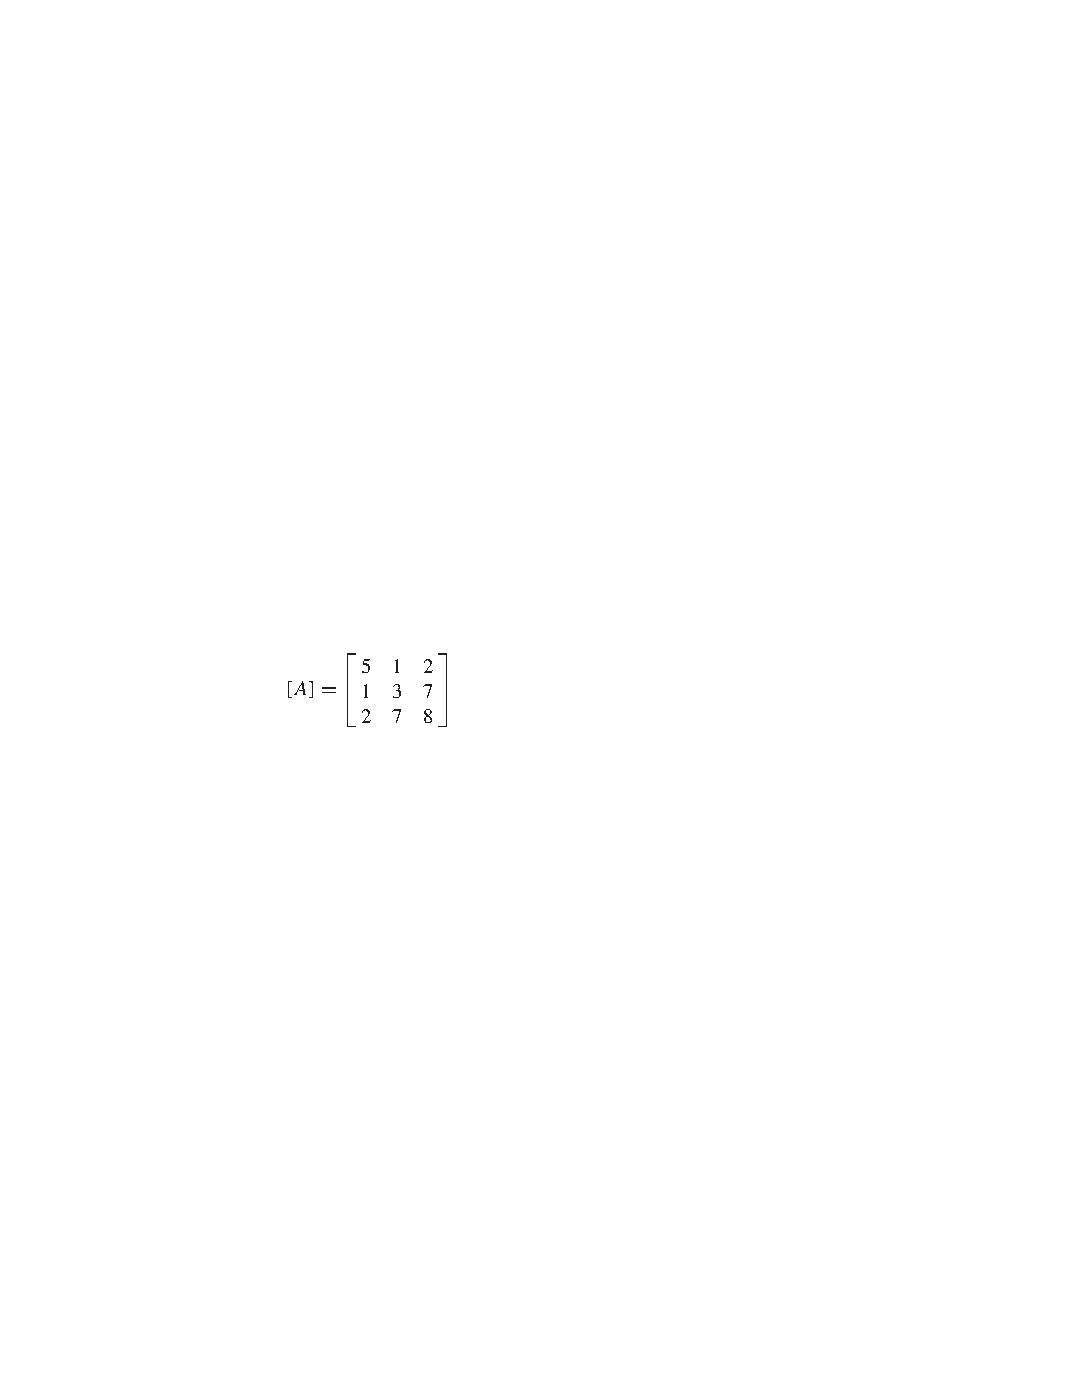
\includegraphics[width=.45\textwidth]{fig/matrix-sym.pdf}
\item <2-> A diagonal matrix :\\
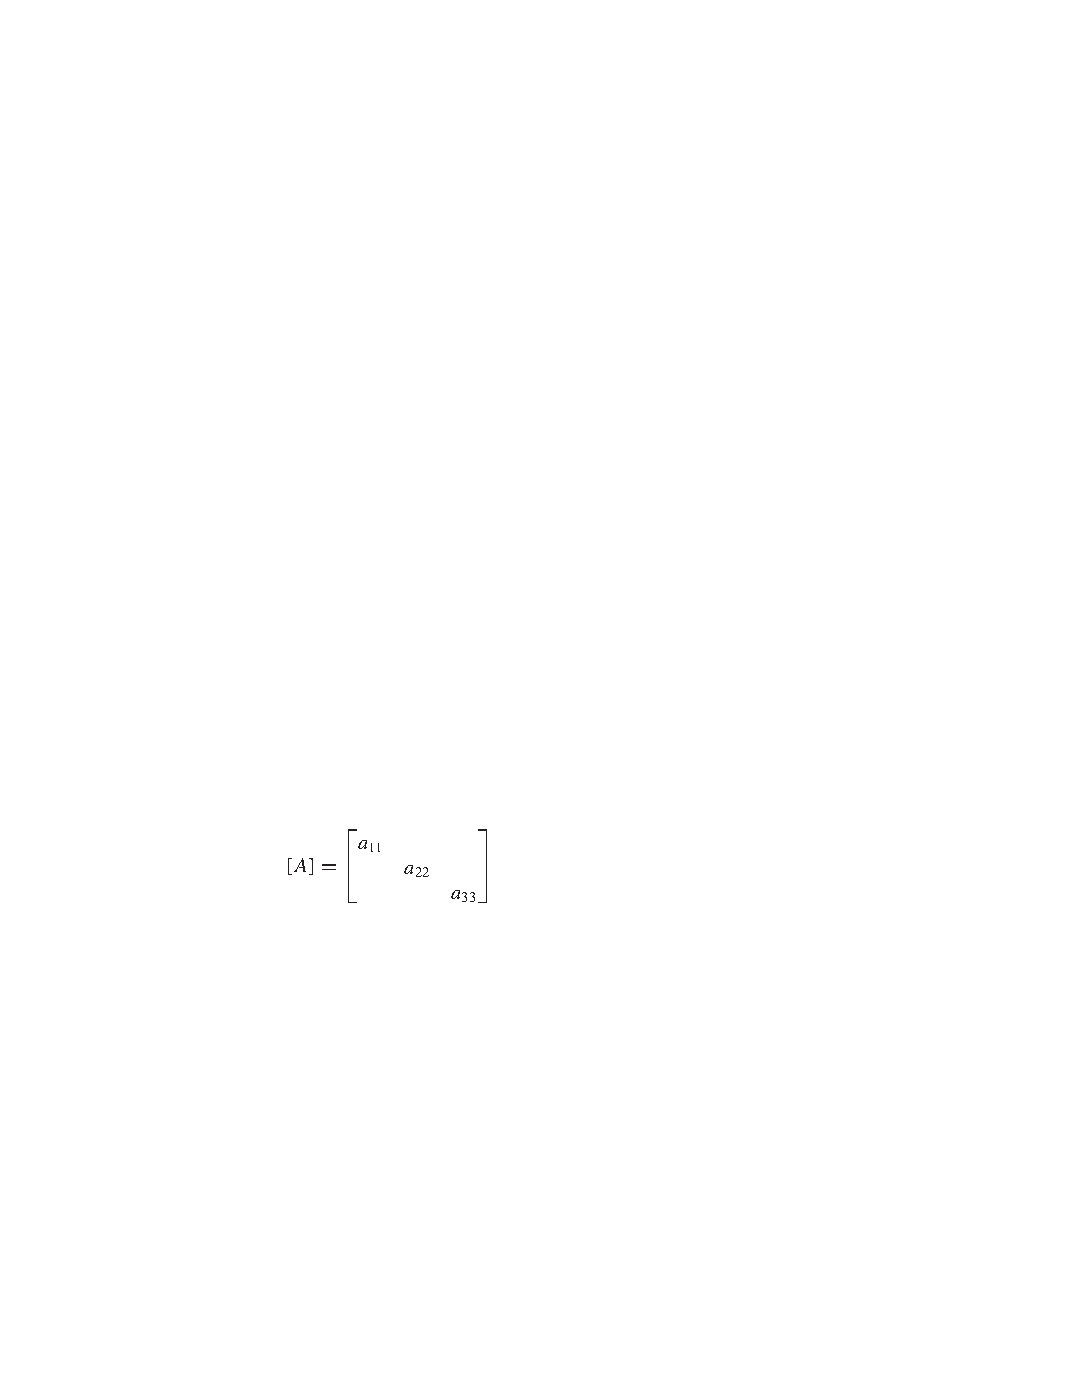
\includegraphics[width=.45\textwidth]{fig/matrix-diag.pdf}
\item <3-> Identity matrix : \\
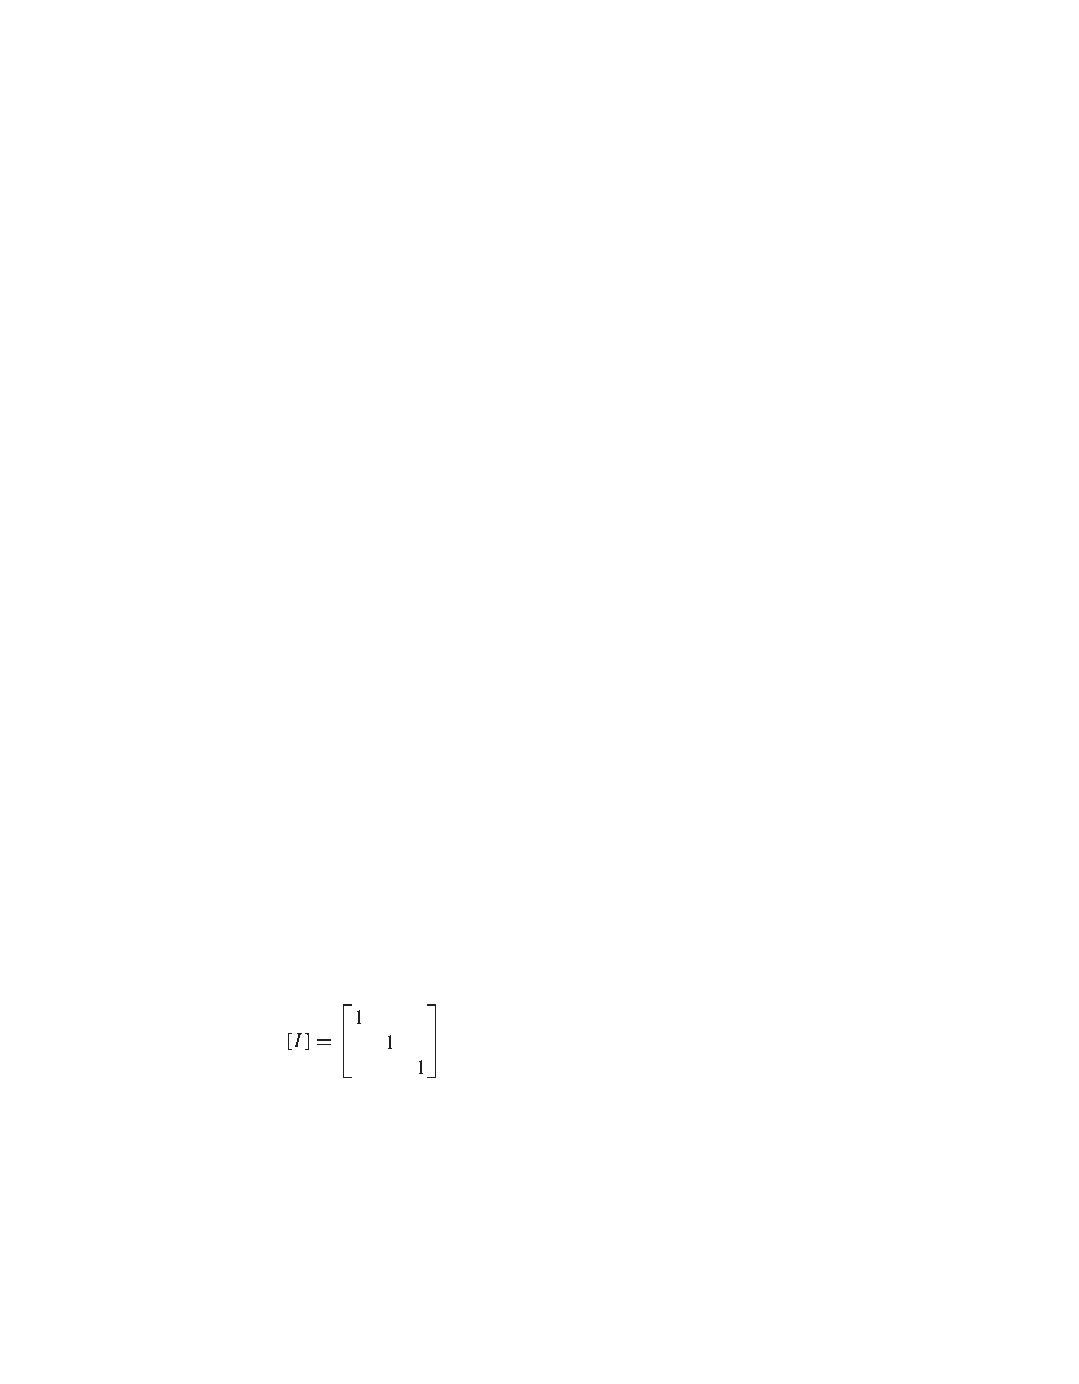
\includegraphics[width=.45\textwidth]{fig/matrix-iden.pdf}
\end{itemize}
\end{block}
\end{column}
\begin{column}{0.45\columnwidth}
\begin{block}{}
\begin{itemize}
\item <4-> Upper triangular :\\
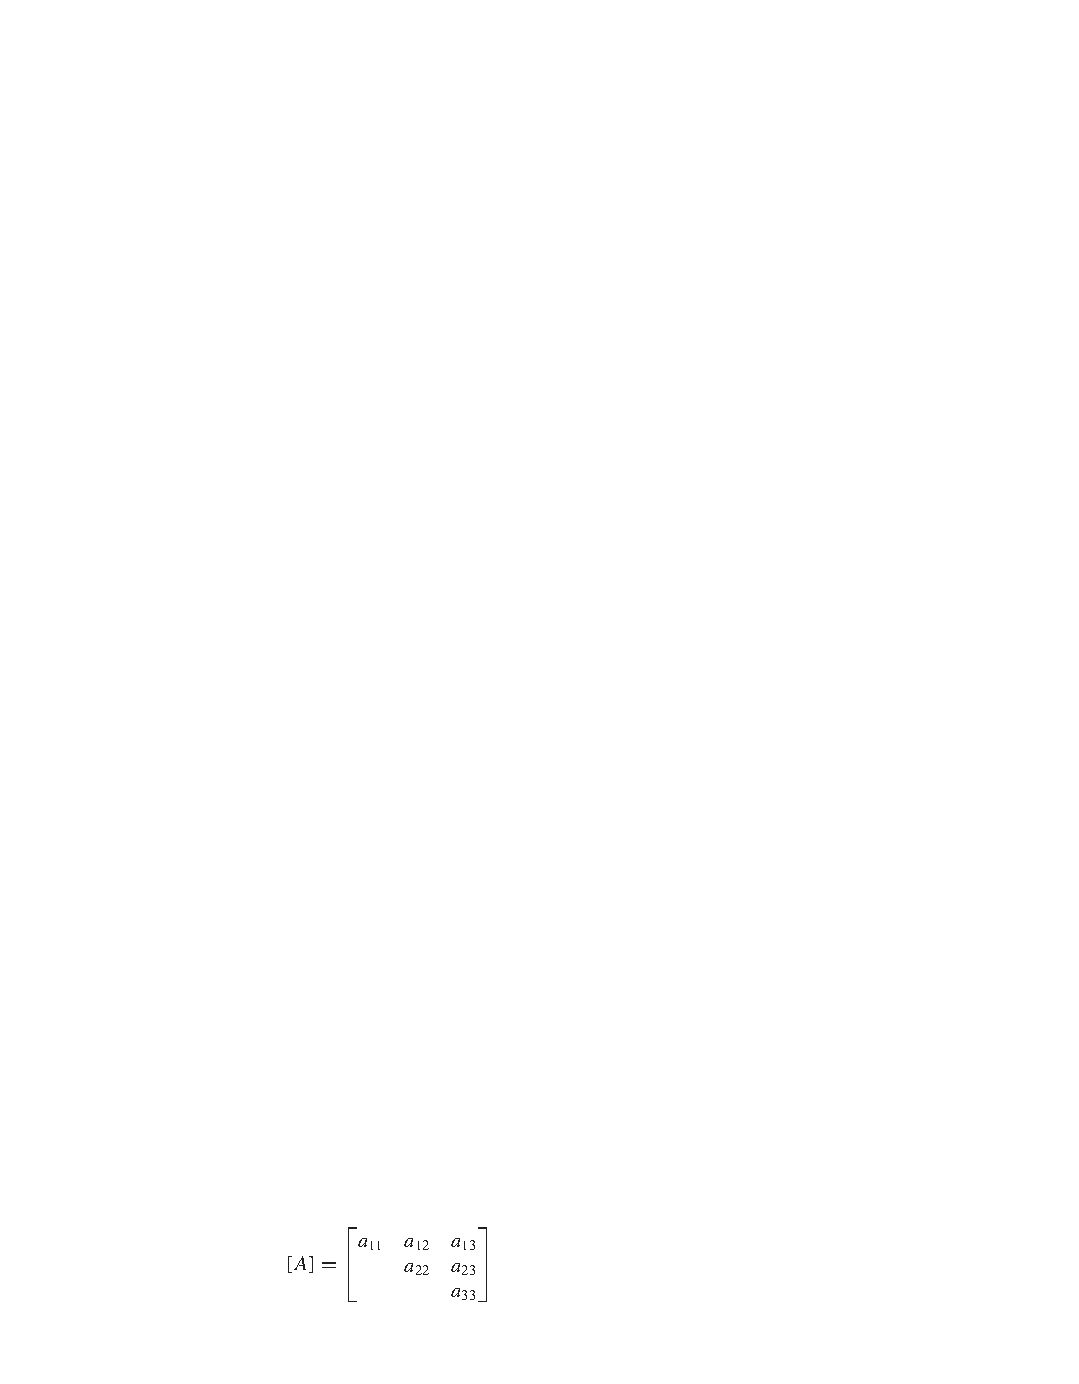
\includegraphics[width=.45\textwidth]{fig/matrix-upper.pdf}
\item <5-> Lower triangular :\\
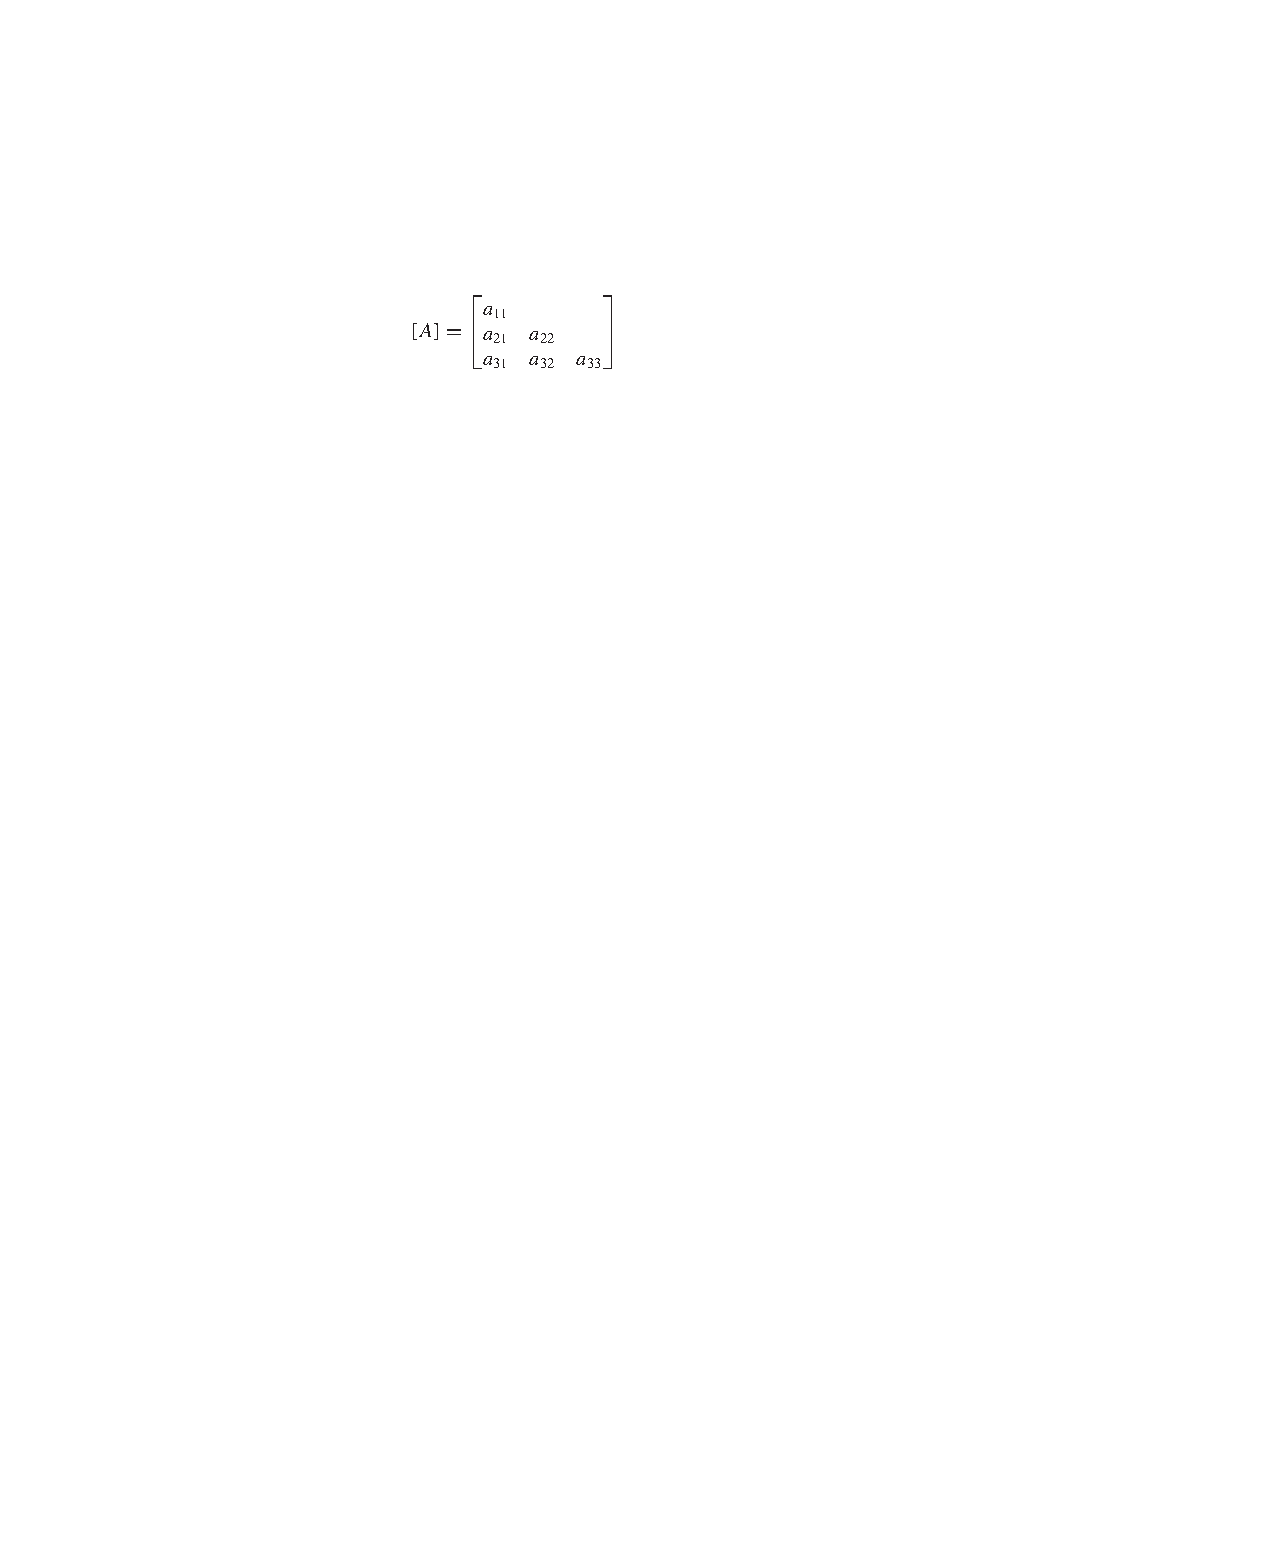
\includegraphics[width=.45\textwidth]{fig/matrix-lower.pdf}
\item <6-> Banded :\\
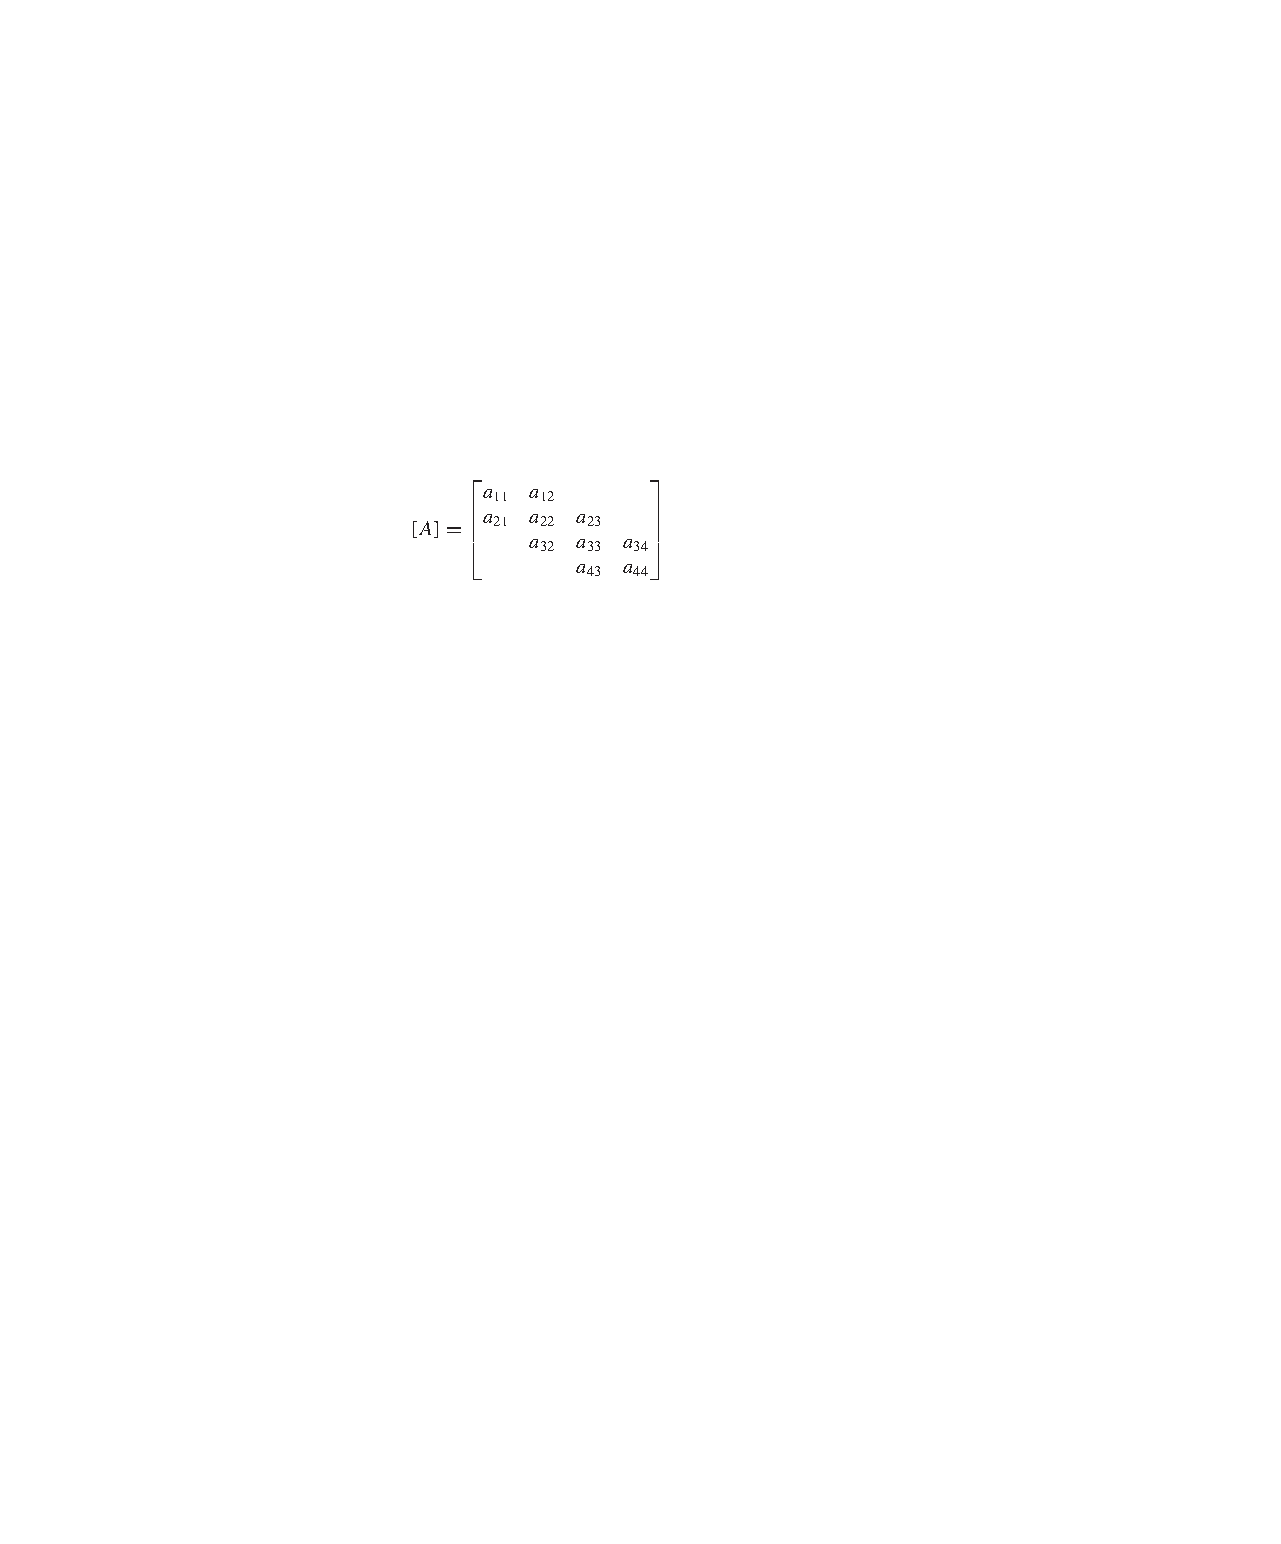
\includegraphics[width=.45\textwidth]{fig/matrix-banded.pdf}
\end{itemize}
\end{block}
\end{column}
\end{columns}
\end{frame}

\begin{frame}[fragile,label={sec:orgb0269ec}]{Matrix definition in python}
 You can use either \texttt{numpy/scipy} or \texttt{sympy}.
\begin{columns}
\begin{column}{0.48\columnwidth}
\begin{block}{See \href{https://docs.scipy.org/doc/numpy-1.14.0/reference/generated/numpy.matrix.html}{numpy docs} .}
\begin{minted}[frame=lines,fontsize=\scriptsize,bgcolor=Wheat!15,escapeinside=||,breaklines=true,breakanywhere=true,bgcolor=Wheat!15,mathescape]{python}
import numpy as np
a = np.matrix('1 2; 3 4')
print(a)
a = np.matrix([[1, 2], [3, 4]])
print(a)
a = np.array([1, 2, 3, 4]).reshape(2,2)
print(a)
\end{minted}

\begin{verbatim}
[[1 2]
 [3 4]]
[[1 2]
 [3 4]]
[[1 2]
 [3 4]]
\end{verbatim}

{\small
\begin{verbatim}
[[1 2]
 [3 4]]
[[1 2]
 [3 4]]
[[1 2]
 [3 4]]
\end{verbatim}
}
\end{block}
\end{column}
\begin{column}{0.48\columnwidth}
\begin{block}{See \href{http://docs.sympy.org/latest/modules/matrices/matrices.html}{sympy docs}}
\begin{minted}[frame=lines,fontsize=\scriptsize,bgcolor=Wheat!15,escapeinside=||,breaklines=true,breakanywhere=true,bgcolor=Wheat!15,mathescape]{python}
from sympy.matrices import Matrix, eye, zeros, ones, diag
M = Matrix([[1,0,4], [0,0,0]])
print(M)
print(eye(4))
print(M[0, 2])
\end{minted}

\begin{verbatim}
Matrix([[1, 0, 4], [0, 0, 0]])
Matrix([[1, 0, 0, 0], [0, 1, 0, 0], [0, 0, 1, 0], [0, 0, 0, 1]])
4
\end{verbatim}

{\small
\begin{verbatim}
Matrix([[1, 0, 4], [0, 0, 0]])
Matrix([[1, 0, 0, 0], [0, 1, 0, 0], [0, 0, 1, 0], [0, 0, 0, 1]])
4
\end{verbatim}
}
\end{block}
\end{column}
\end{columns}
\end{frame}

\begin{frame}[fragile,label={sec:org23bc246}]{Matrix operations in python}
 \begin{columns}
\begin{column}{0.50\columnwidth}
\begin{block}{Example in python}
\begin{minted}[frame=lines,fontsize=\scriptsize,bgcolor=Wheat!15,escapeinside=||,breaklines=true,breakanywhere=true,bgcolor=Wheat!15,mathescape]{python}
import numpy as np
a = np.matrix('1 2; 3 4')
b = np.matrix([[5, -1], [-3, 24]])
c = a+b # sum
print(c)
c = a*b # Multiplication
print(c)
c = a/b # multiply by the inverse of b
print(c)
print(c.max())
print(c.min())
d = np.array([[5, -1], [-3, 24]])
print("d:\n",d)
\end{minted}
\end{block}
\end{column}

\begin{column}{0.45\columnwidth}
\begin{block}{Output}
\begin{verbatim}
    [[ 6  1]
     [ 0 28]]
    [[-1 47]
     [ 3 93]]
    [[ 0.2        -2.        ]
     [-1.          0.16666667]]
    0.2
    -2.0
    d:
     [[ 5 -1]
     [-3 24]]
\end{verbatim}
\end{block}
\end{column}
\end{columns}
\end{frame}

\begin{frame}[standout,label=]{}
You can watch : \url{https://www.youtube.com/watch?v=XkY2DOUCWMU}
\end{frame}

\section{Solving linear systems \(Ax = b\)}
\label{sec:org324b4f0}
\begin{frame}[fragile,label={sec:org865dd59}]{Example}
 Solve the following linear system  (See \href{https://docs.scipy.org/doc/numpy/reference/generated/numpy.linalg.solve.html}{numpy linalg}) \\

\begin{figure}[H]


\includegraphics[width=0.6\textwidth]{fig/linear-example-01.pdf}
\end{figure}

\pause

\begin{minted}[frame=lines,fontsize=\scriptsize,bgcolor=Wheat!15,escapeinside=||,breaklines=true,breakanywhere=true,bgcolor=Wheat!15,mathescape]{python}
import numpy as np

A = np.array([[150, -100, 0], [-100, 150, -50], [0, -50, 50]])
b = np.array([588.6, 686.7, 784.8])
x = np.linalg.solve(A, b) # magic
print(x)
# confirm
print(A.dot(x) - b)
\end{minted}
\pause
{\vspace*{-4ex}\small
\begin{verbatim}
[41.202 55.917 71.613]
[1.25055521e-12 6.82121026e-13 2.27373675e-13]
\end{verbatim}
}
\end{frame}

\begin{frame}[label={sec:org5ebc52c}]{Exercise 1}
\begin{figure}[H]

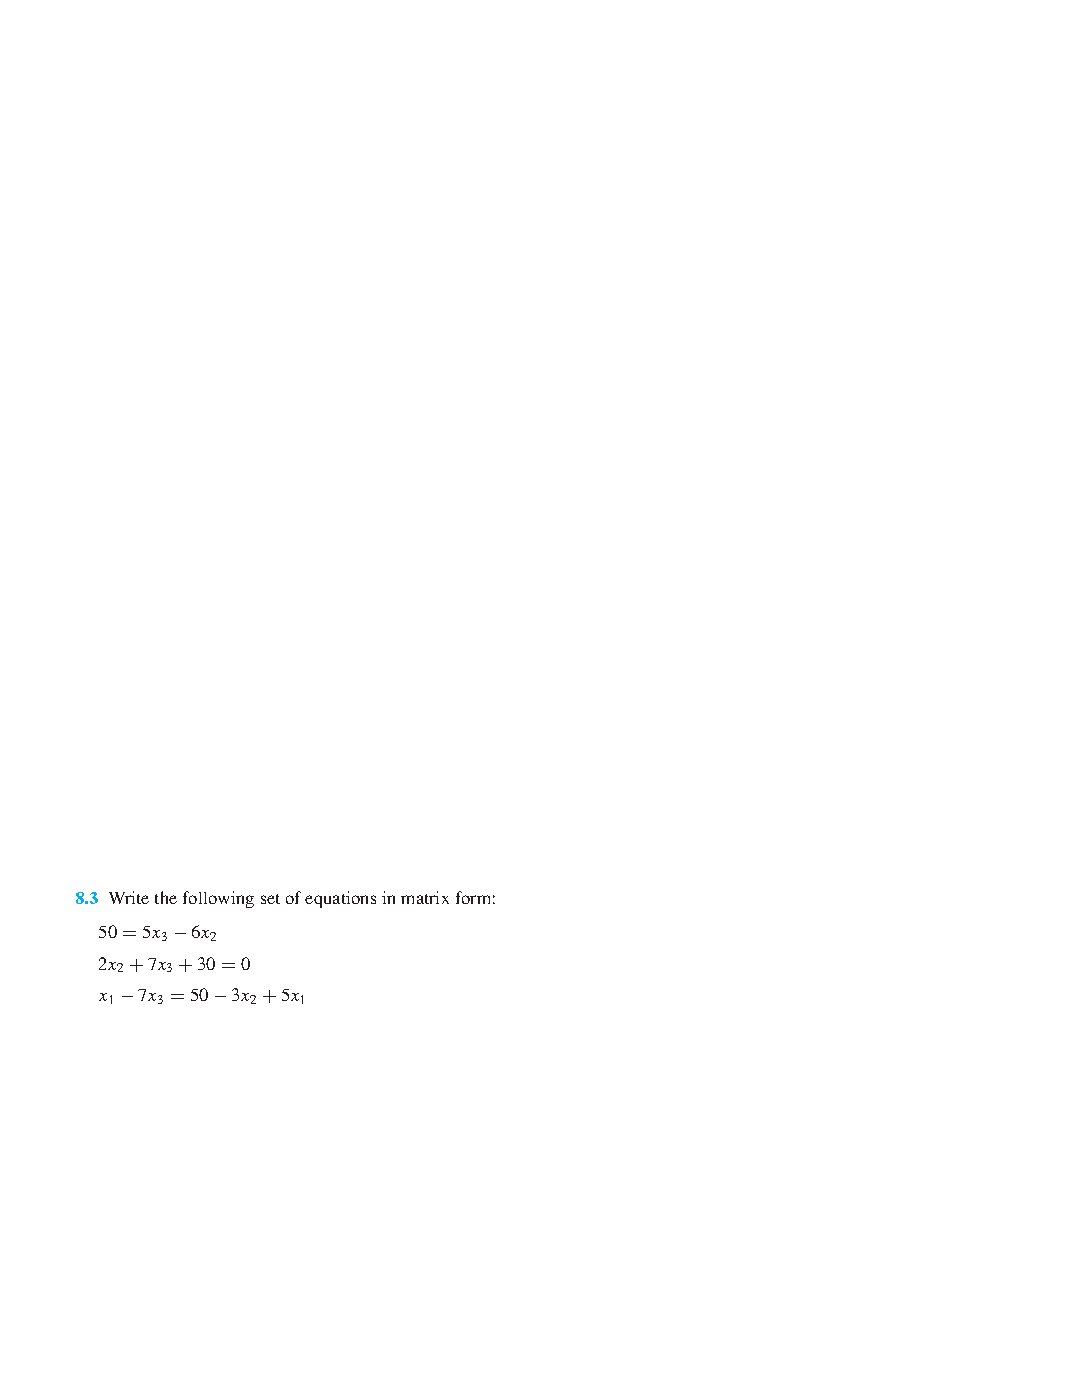
\includegraphics[width=0.9\textwidth]{fig/linear-example-03.pdf}
\end{figure}   

Solve the system. 
\end{frame}

\begin{frame}[label={sec:org93a0e53}]{Exercise 2}
Solve the following system\\
\begin{figure}[H]

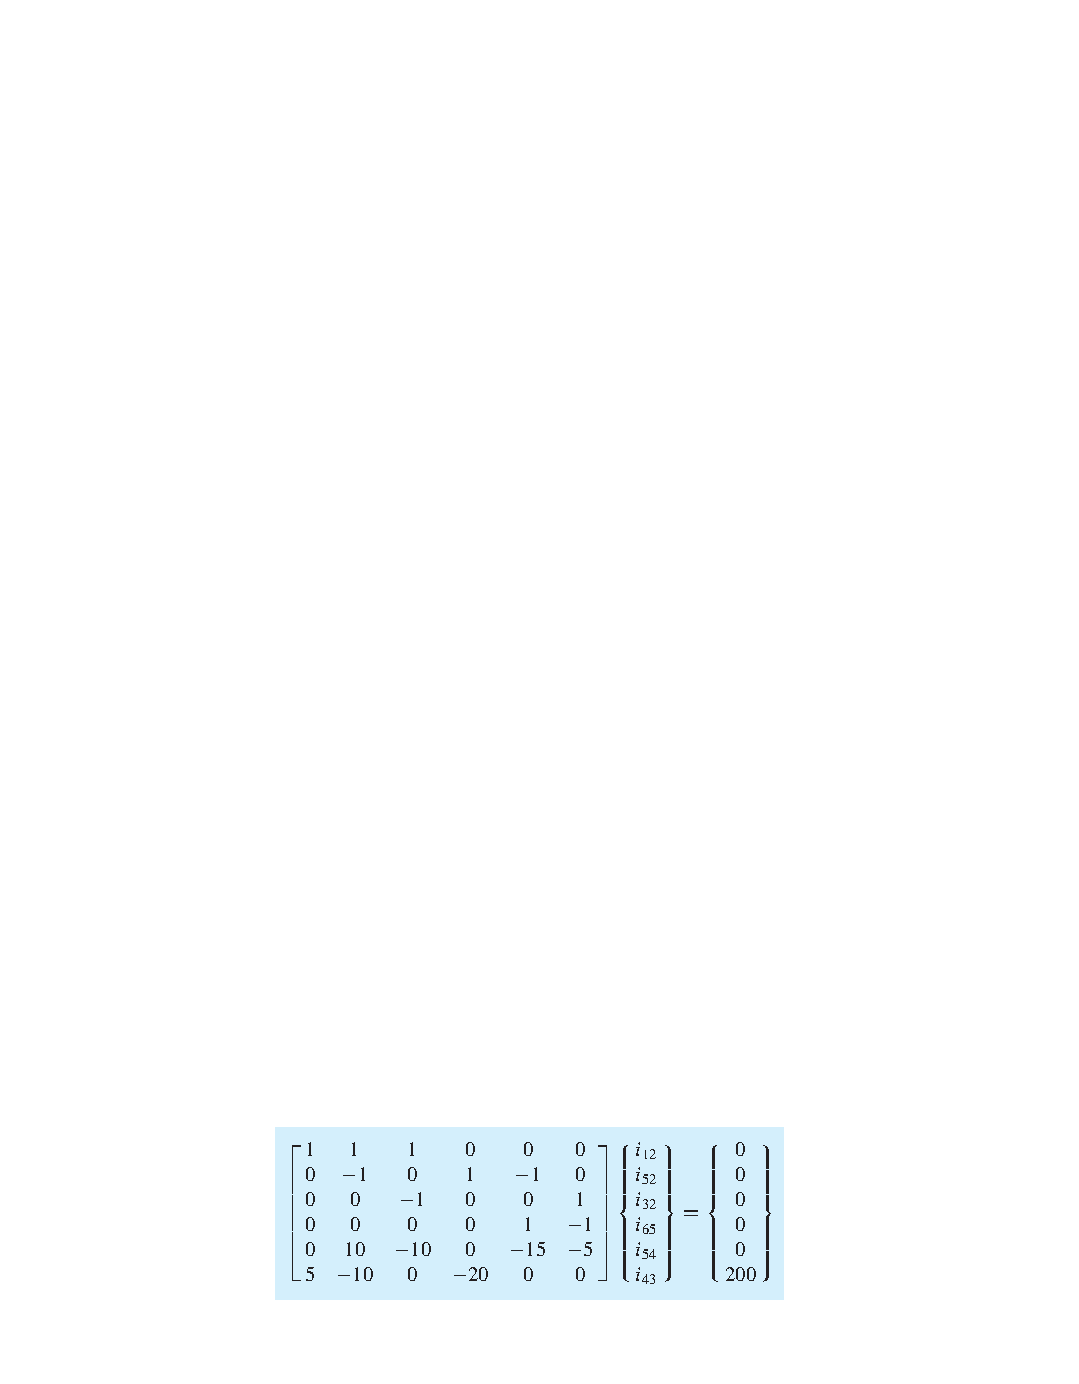
\includegraphics[width=0.6\textwidth]{fig/linear-example-02.pdf}
\end{figure}

Can you measure the time spent?
\end{frame}
\begin{frame}[label={sec:org1e9e864}]{Exercise 3}
\vfill\vfill
Solve this system: 
$$ \frac{-2.3x_1}{5} + x_2 = 1.1 $$
$$-0.5x_1 + x_2 = 1 $$
\vfill
Plot the system of equations and check whether this solution is or
not special.
\vfill
\end{frame}

\begin{frame}[label={sec:org81f1c07}]{Exercise 4: Simulating temperature}
\vfill
\begin{figure}[H]

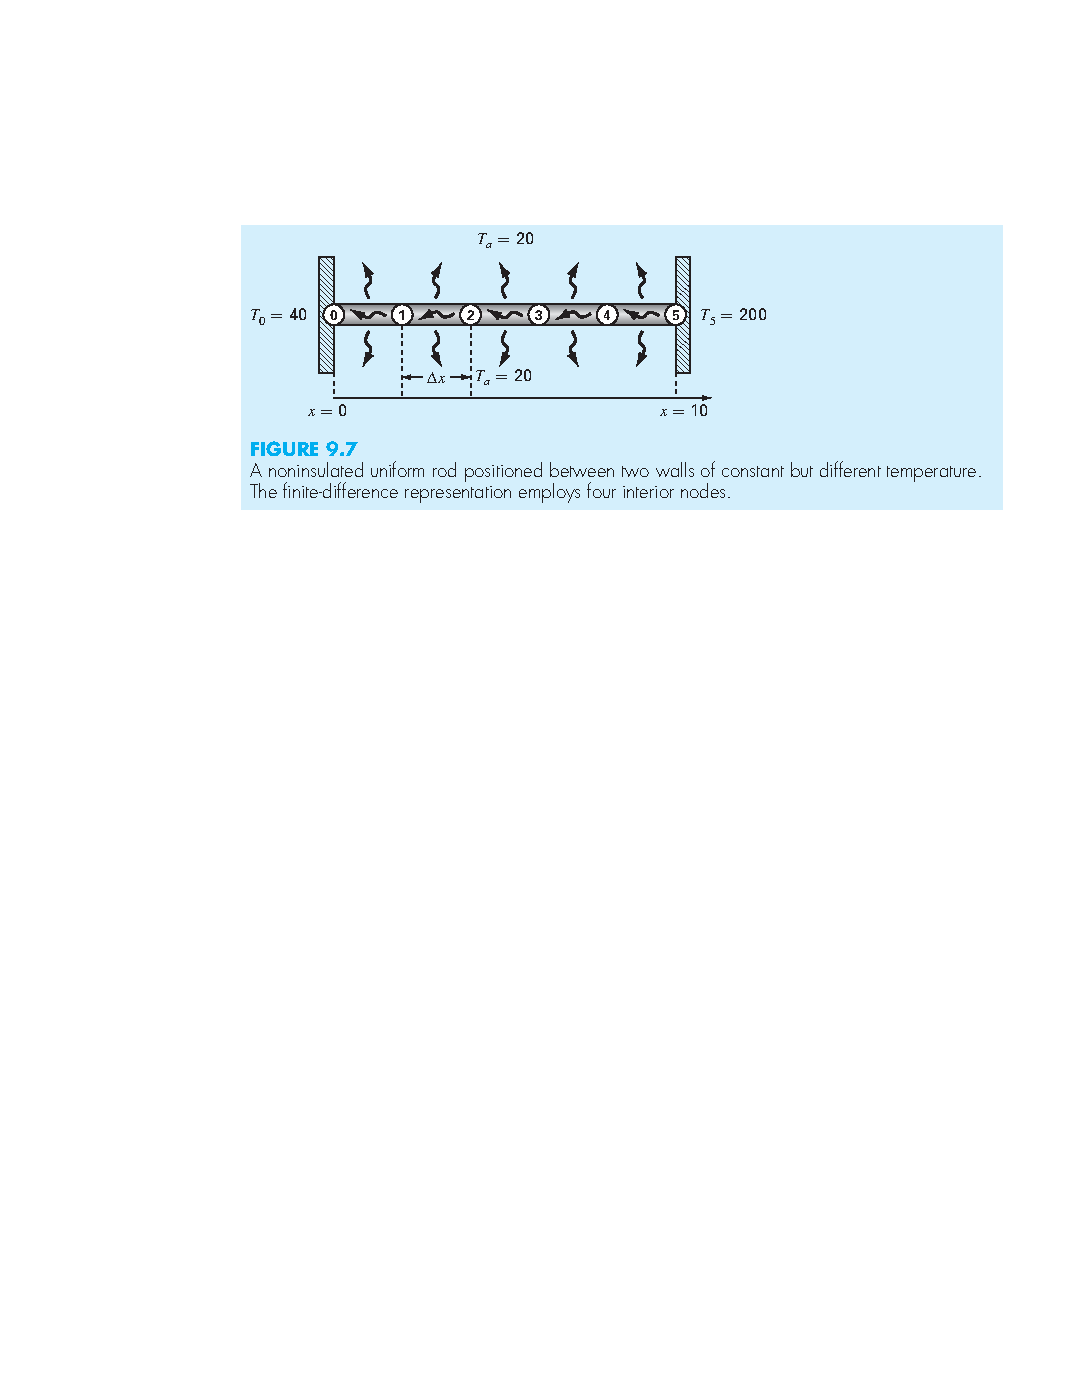
\includegraphics[width=0.8\textwidth]{fig/linear-example-04-T.pdf}
\end{figure}

\begin{figure}[H]

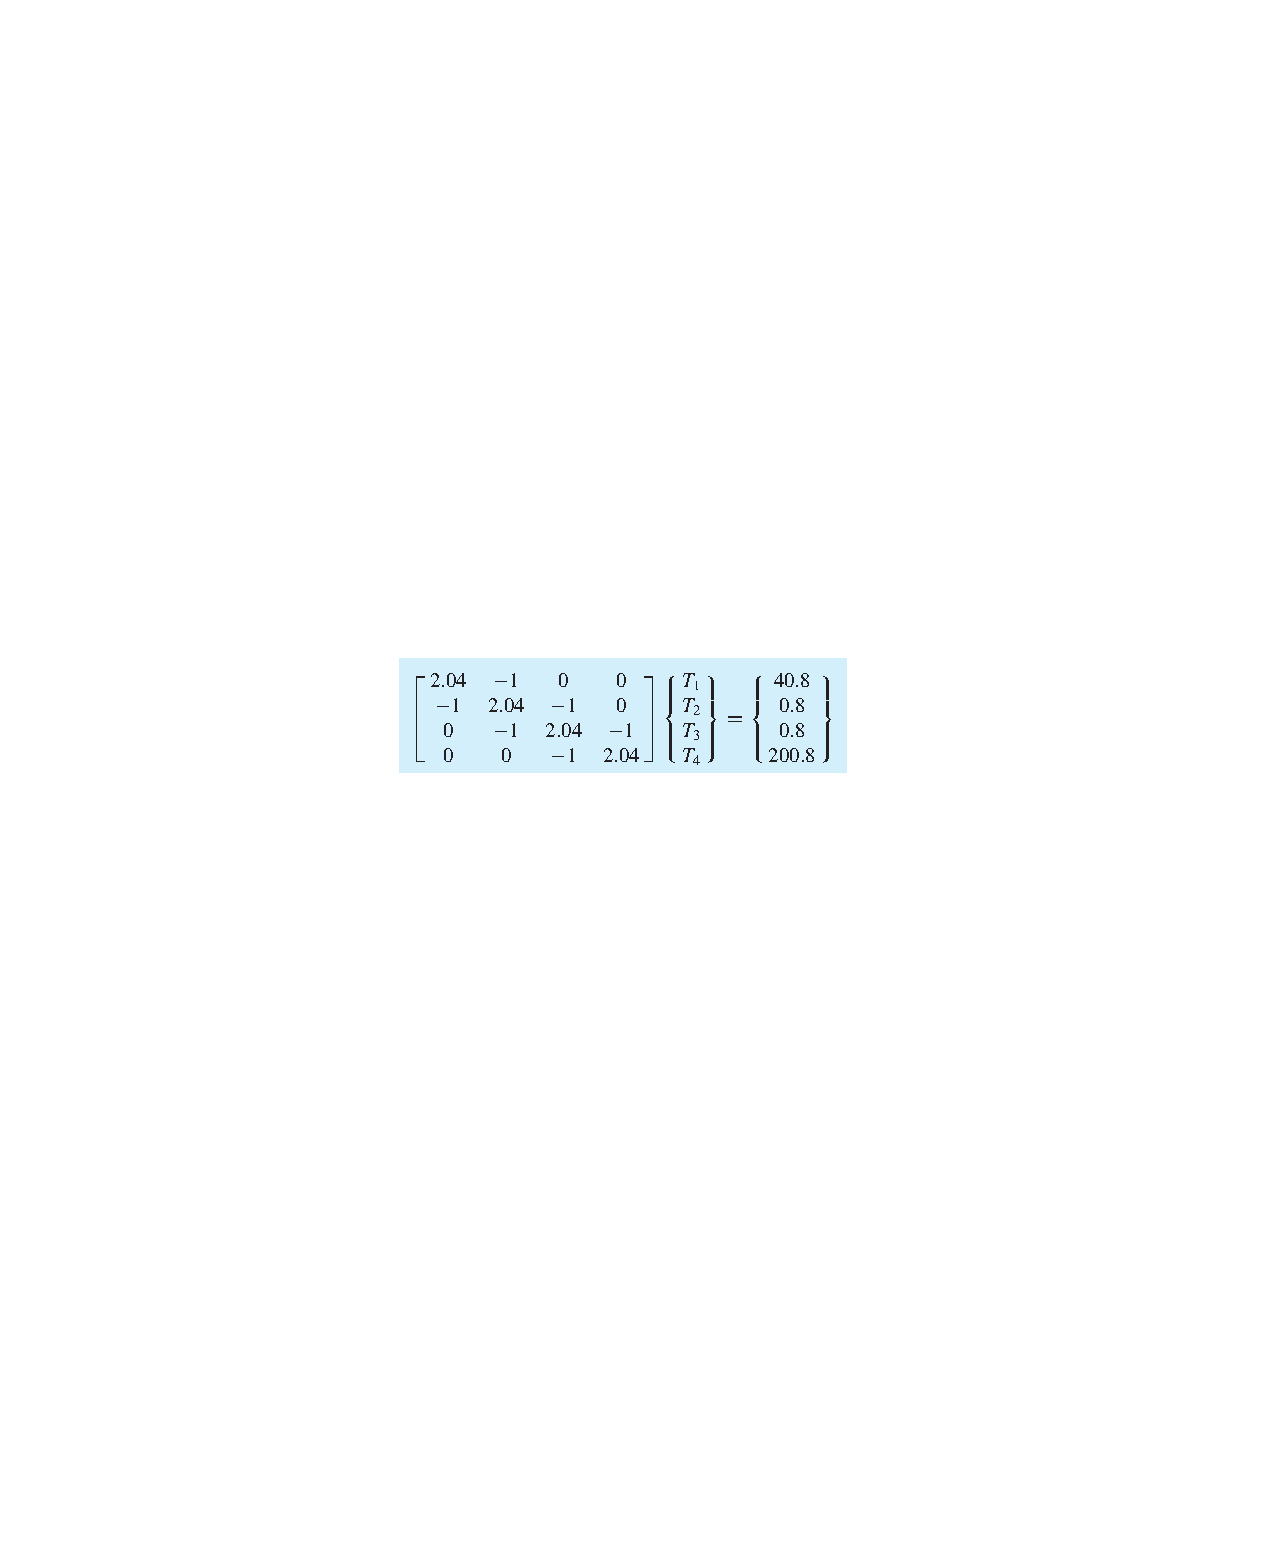
\includegraphics[width=0.8\textwidth]{fig/linear-example-04-T-B.pdf}
\end{figure}
\vfill
\end{frame}

\begin{frame}[standout,label=]{}
\end{frame}
\section{Computing the determinant}
\label{sec:org7ba0c82}
\begin{frame}[fragile,label={sec:org60dad40}]{Using \texttt{scipy}}
 See the \href{https://docs.scipy.org/doc/scipy/reference/generated/scipy.linalg.det.html\#scipy.linalg.det}{docs for determinant}
\pause
\begin{minted}[frame=lines,fontsize=\scriptsize,bgcolor=Wheat!15,escapeinside=||,breaklines=true,breakanywhere=true,bgcolor=Wheat!15,mathescape]{python}
from scipy import linalg
import numpy as np
A = np.array([[1,2,3], [4,5,6], [7,8,9]])
print(linalg.det(A))
A = np.array([[0,2,3], [4,5,6], [7,8,9]])
print(linalg.det(A))
\end{minted}
\pause

\begin{verbatim}
0.0
3.0
\end{verbatim}

You can watch : \url{https://www.youtube.com/watch?v=Ip3X9LOh2dk}
\end{frame}
\begin{frame}[label={sec:org7a1bb2d}]{Exercise 1}
\begin{figure}[H]

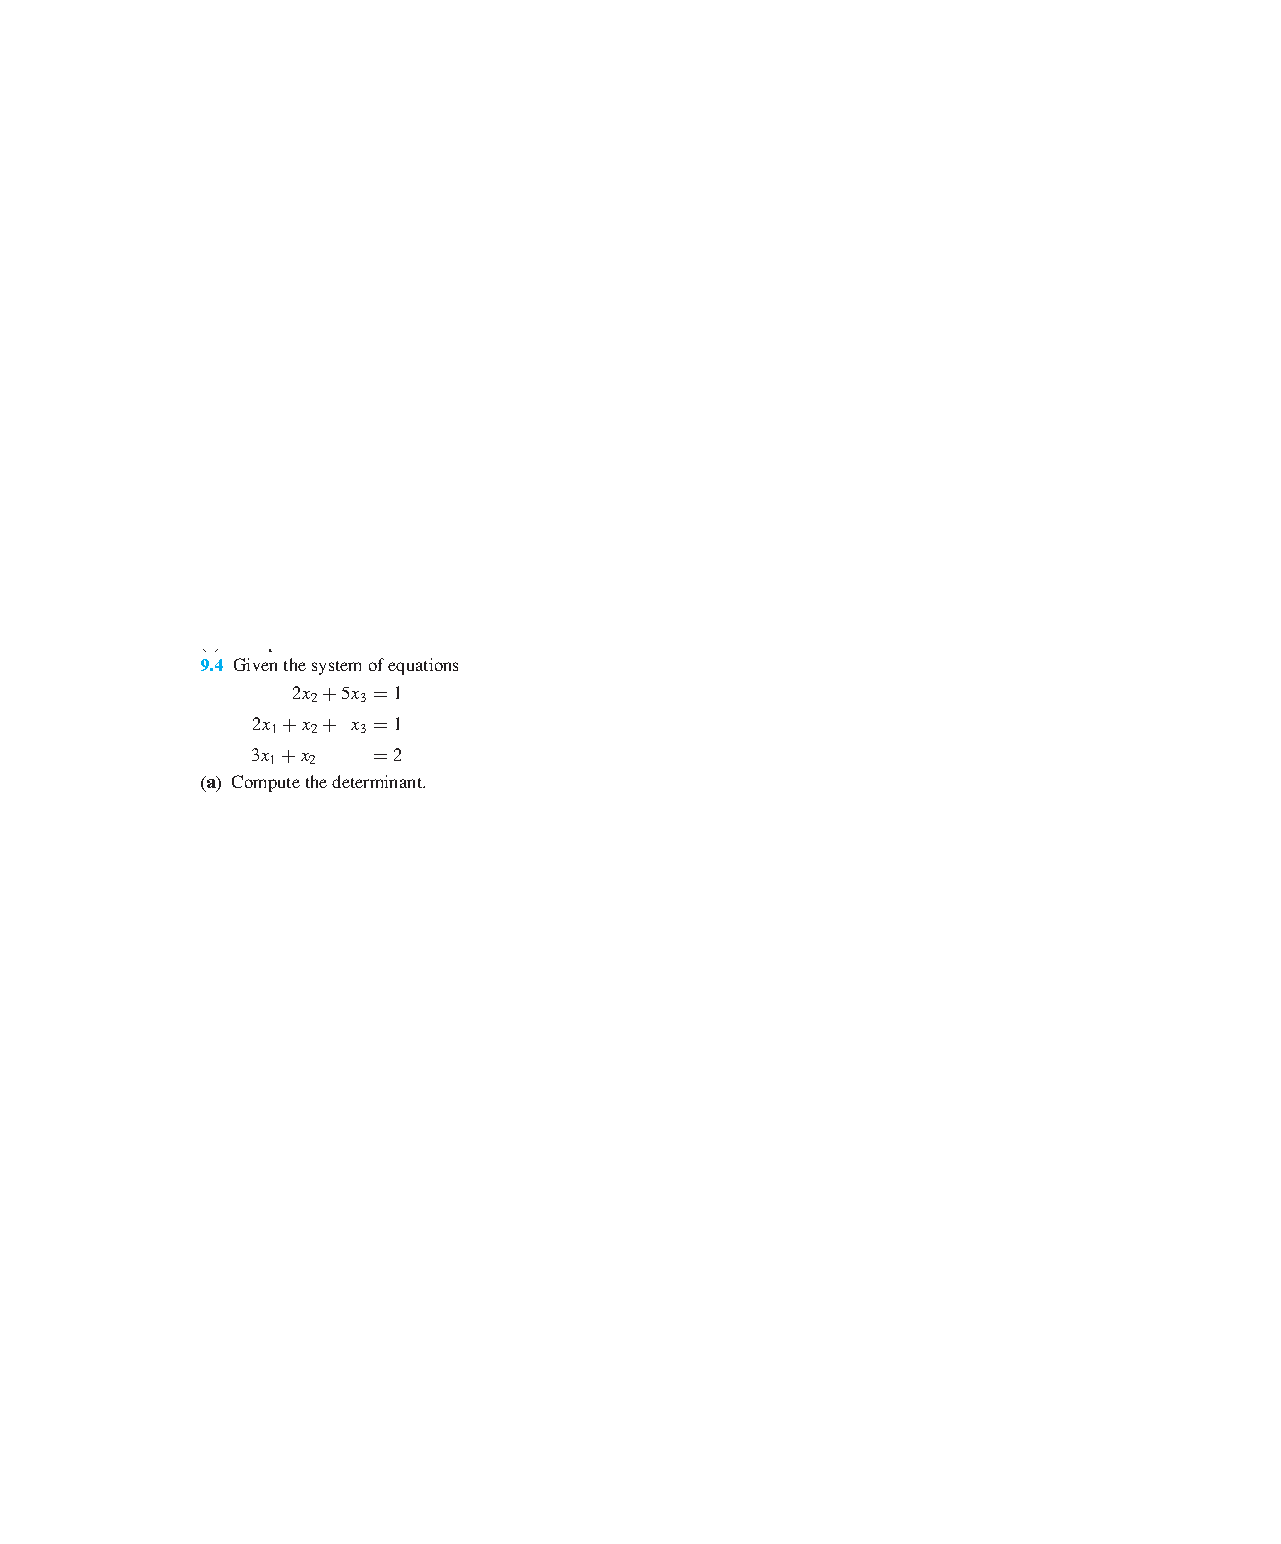
\includegraphics[width=0.9\textwidth]{fig/det-01.pdf}
\end{figure}
\end{frame}

\begin{frame}[standout,label=]{}
\end{frame}
\section{Computing the inverse}
\label{sec:org7598823}
\begin{frame}[fragile,label={sec:org2d22ade}]{Using \texttt{scipy}}
 See \href{https://docs.scipy.org/doc/scipy/reference/generated/scipy.linalg.inv.html\#scipy.linalg.inv}{inverse with \texttt{scipy}}
\begin{minted}[frame=lines,fontsize=\scriptsize,bgcolor=Wheat!15,escapeinside=||,breaklines=true,breakanywhere=true,bgcolor=Wheat!15,mathescape]{python}
from scipy import linalg
import numpy as np
A = np.array([[1., 2.], [3., 4.]])
B = linalg.inv(A)
print(B)
# verify
print(A.dot(B))
\end{minted}

\begin{verbatim}
[[-2.   1. ]
 [ 1.5 -0.5]]
[[1.0000000e+00 0.0000000e+00]
 [8.8817842e-16 1.0000000e+00]]
\end{verbatim}


You can watch: \url{https://www.youtube.com/watch?v=uQhTuRlWMxw}
\end{frame}
\begin{frame}[label={sec:org34c3fd6}]{Condition number}
\vfill
The number
\(\kappa = ||A|| ||A^{-1}||\)
is called the condition number of a matrix. Ideally it is \(1\). If \(\kappa\) is much
larger than one, the matrix is ill-conditioned and the solution
might have a lot of error.
\vfill
Compute the condition number of the following matrix:

\begin{equation}
A = 
\begin{bmatrix}
1.001 & 0.001\\
0.000 & 0.999
\end{bmatrix}
\end{equation}
\vfill
\end{frame}
\begin{frame}[standout,label=]{}
\end{frame}
\section{Matrix factorizations}
\label{sec:orgec72e6c}
\begin{frame}[fragile,label={sec:org50a5e5b}]{LU}
 You can specifically solve with LU factorization. See \href{https://docs.scipy.org/doc/scipy/reference/generated/scipy.linalg.lu\_solve.html\#scipy.linalg.lu\_solve}{docs} .
\begin{minted}[frame=lines,fontsize=\scriptsize,bgcolor=Wheat!15,escapeinside=||,breaklines=true,breakanywhere=true,bgcolor=Wheat!15,mathescape]{python}
from scipy.linalg import lu_factor, lu_solve
import numpy as np
A = np.array([[2, 5, 8, 7], [5, 2, 2, 8], [7, 5, 6, 6], [5, 4, 4, 8]])
b = np.array([1, 1, 1, 1])
lu, piv = lu_factor(A)
x = lu_solve((lu, piv), b)
print(x)
print(A.dot(x) - b)
\end{minted}

\begin{verbatim}
[ 0.05154639 -0.08247423  0.08247423  0.09278351]
[0. 0. 0. 0.]
\end{verbatim}
\end{frame}
\begin{frame}[fragile,label={sec:orga2f8aa5}]{Cholesky}
 Or you can use the Cholesky factorization. 
See \href{https://docs.scipy.org/doc/scipy/reference/generated/scipy.linalg.cho\_solve.html\#scipy.linalg.cho\_solve}{Cholesky docs} . The matrix must be positive definite. 
\begin{minted}[frame=lines,fontsize=\scriptsize,bgcolor=Wheat!15,escapeinside=||,breaklines=true,breakanywhere=true,bgcolor=Wheat!15,mathescape]{python}
from scipy.linalg import cho_factor, cho_solve
import numpy as np
A = np.array([[9, 3, 1, 5], [3, 7, 5, 1], [1, 5, 9, 2], [5, 1, 2, 6]])
b = np.array([1, 1, 1, 1])
c, low = cho_factor(A)
x = cho_solve((c, low), b)
print(x)
print(A.dot(x) - b)
\end{minted}

\begin{verbatim}
[-0.01749271  0.11953353  0.01166181  0.1574344 ]
[2.22044605e-16 2.22044605e-16 0.00000000e+00 0.00000000e+00]
\end{verbatim}
\end{frame}

\begin{frame}[standout,label=]{}
\end{frame}
\section{Eigen value and eigen vectors}
\label{sec:org693ffc9}
\begin{frame}[label={sec:orgb97294f}]{Definition}
\vfill
The eigen-values and eigen-vectors of a matrix satisfy the equation 

$$ Ax = \lambda x $$


The eigen-vectors form a basis where the matrix can be
diagonalized. In general, computing the eigen vectors and
aeigenvalues is hard, and they can also be complex.
\vfill

You can watch: \url{https://www.youtube.com/watch?v=PFDu9oVAE-g}
\end{frame}
\begin{frame}[fragile,label={sec:org7408179}]{Implementation in Python}
 See \href{https://docs.scipy.org/doc/scipy/reference/generated/scipy.linalg.eig.html\#scipy.linalg.eig}{docs for scipy}

\begin{minted}[frame=lines,fontsize=\scriptsize,bgcolor=Wheat!15,escapeinside=||,breaklines=true,breakanywhere=true,bgcolor=Wheat!15,mathescape]{python}
import numpy as np
from scipy import linalg
A = np.array([[0., -1.], [1., 0.]])
#A = np.array([[1, 0.], [0., 2.]])
#A = np.array([[2, 5, 8, 7], [5, 2, 2, 8], [7, 5, 6, 6], [5, 4, 4, 8]])
#A = np.array([[2, 5, 8, 7], [5, 2, 2, 8], [7, 5, 6, 6], [5, 4, 4, 8]])
sol = linalg.eig(A)
print("Eigen-values: ", sol[0])
print("Eigen-vectors:\n", sol[1])
# verify
print("Verification: ", A.dot(sol[1][:, 0]) - sol[0][0]*sol[1][:, 0])
\end{minted}

{\scriptsize
\begin{verbatim}
Eigen-values:  [0.+1.j 0.-1.j]
Eigen-vectors:
 [[0.70710678+0.j         0.70710678-0.j        ]
 [0.        -0.70710678j 0.        +0.70710678j]]
Verification:  [0.+0.j 0.+0.j]
\end{verbatim}
}
\end{frame}
\begin{frame}[label={sec:org3b7fe13}]{Exercise 1 \cite{cheney2012numerical}}
\vfill
\begin{figure}[H]

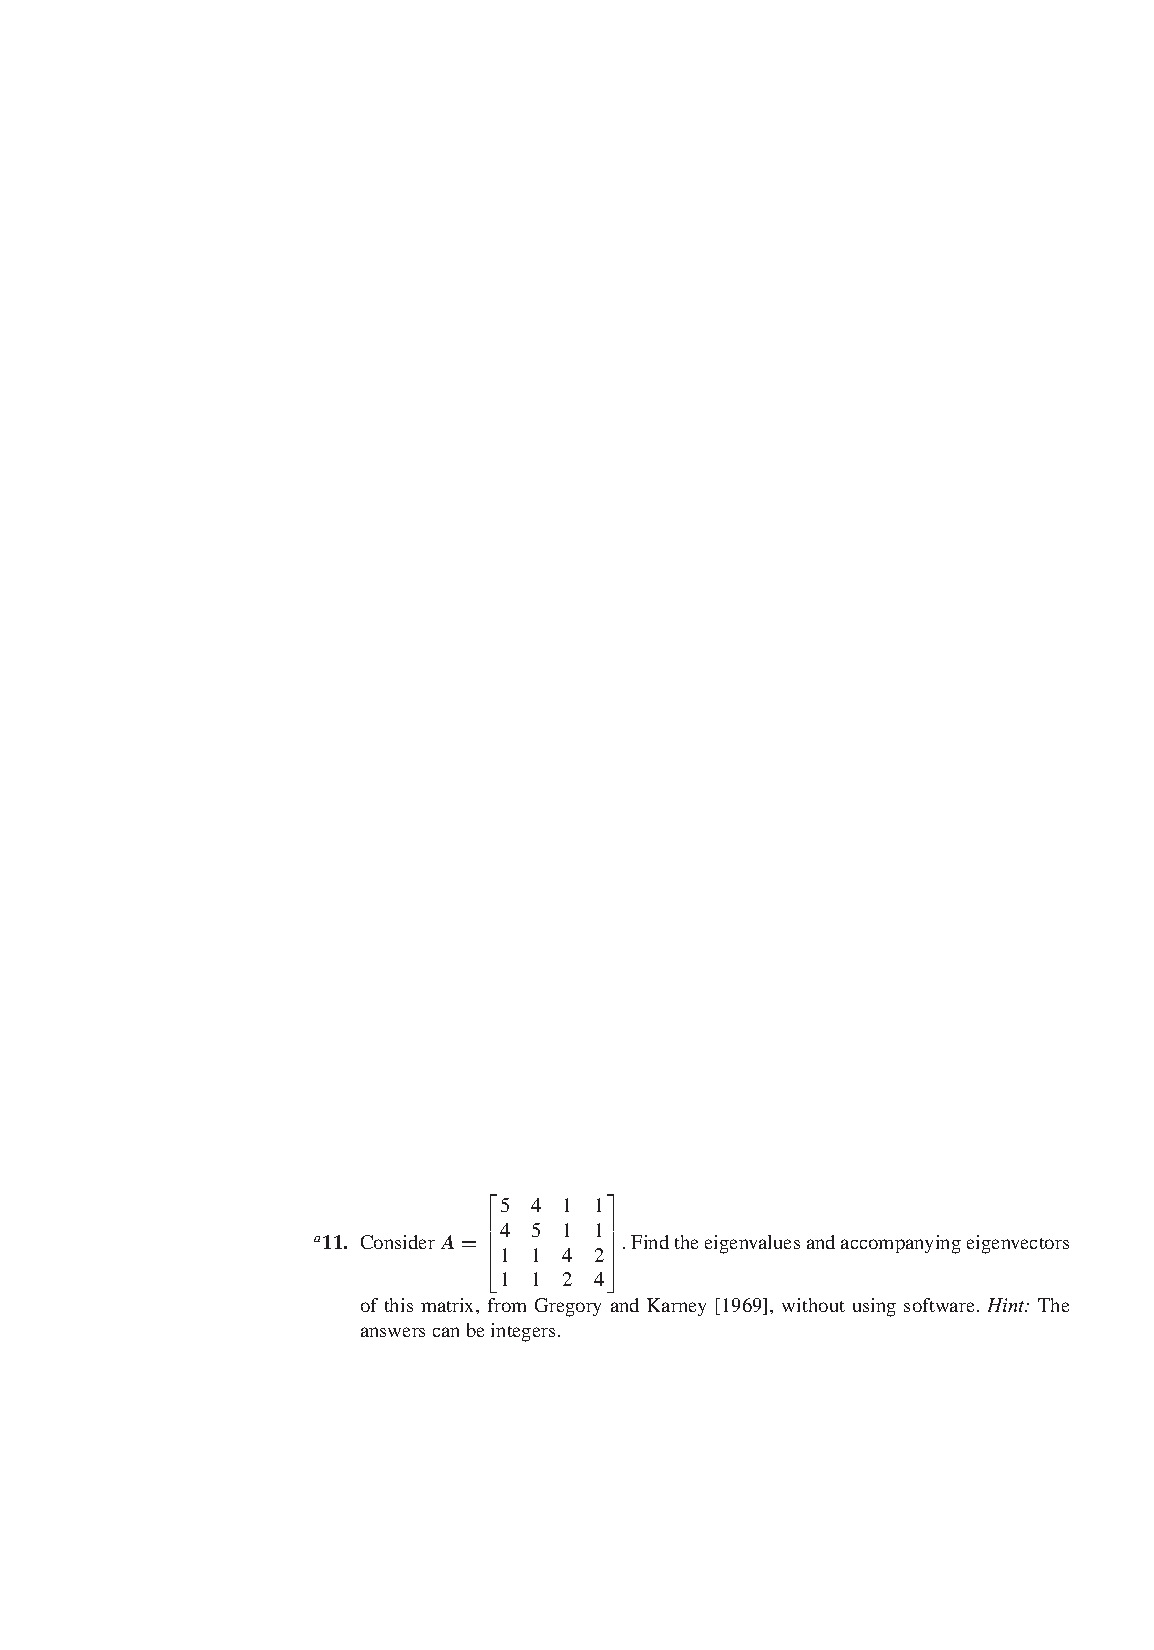
\includegraphics[width=1.0\textwidth]{fig/eigen-exer-02.pdf}
\end{figure}
\vfill
\end{frame}
\begin{frame}[standout,label=]{}
\end{frame}
\section{Problems}
\label{sec:orgf9c5e7b}
\begin{frame}[label={sec:orgf410e4a}]{Problem 1}
\vfill
Create a random matrix, with random elements between [-1, 1], and
make a histogram for the largest eigenvalue.
\vfill
\end{frame}
\begin{frame}[label={sec:org9e7710c}]{Problem 2 \cite{cheney2012numerical}}
\begin{figure}[H]

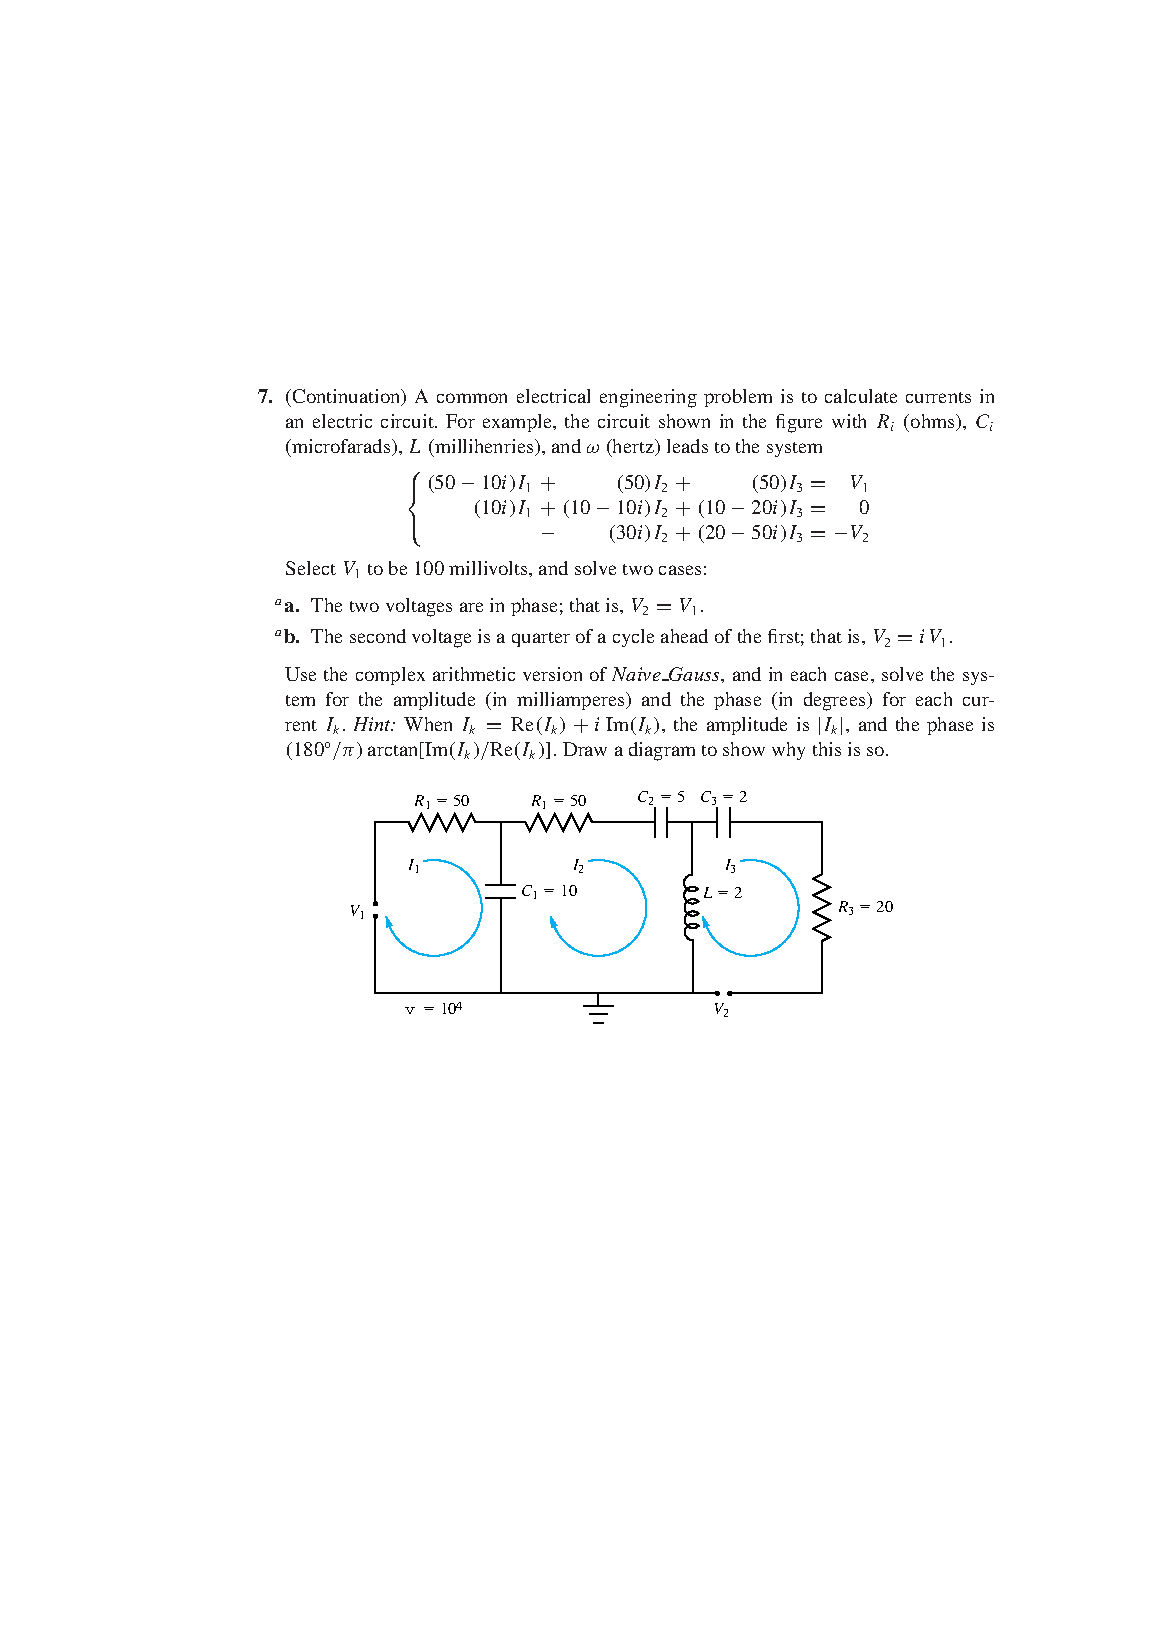
\includegraphics[width=0.8\textwidth]{fig/problem-01.pdf}
\end{figure}
\end{frame}

\begin{frame}[label={sec:org6a826ca}]{Problem 3 \cite{cheney2012numerical}}
\vfill
\begin{figure}[H]

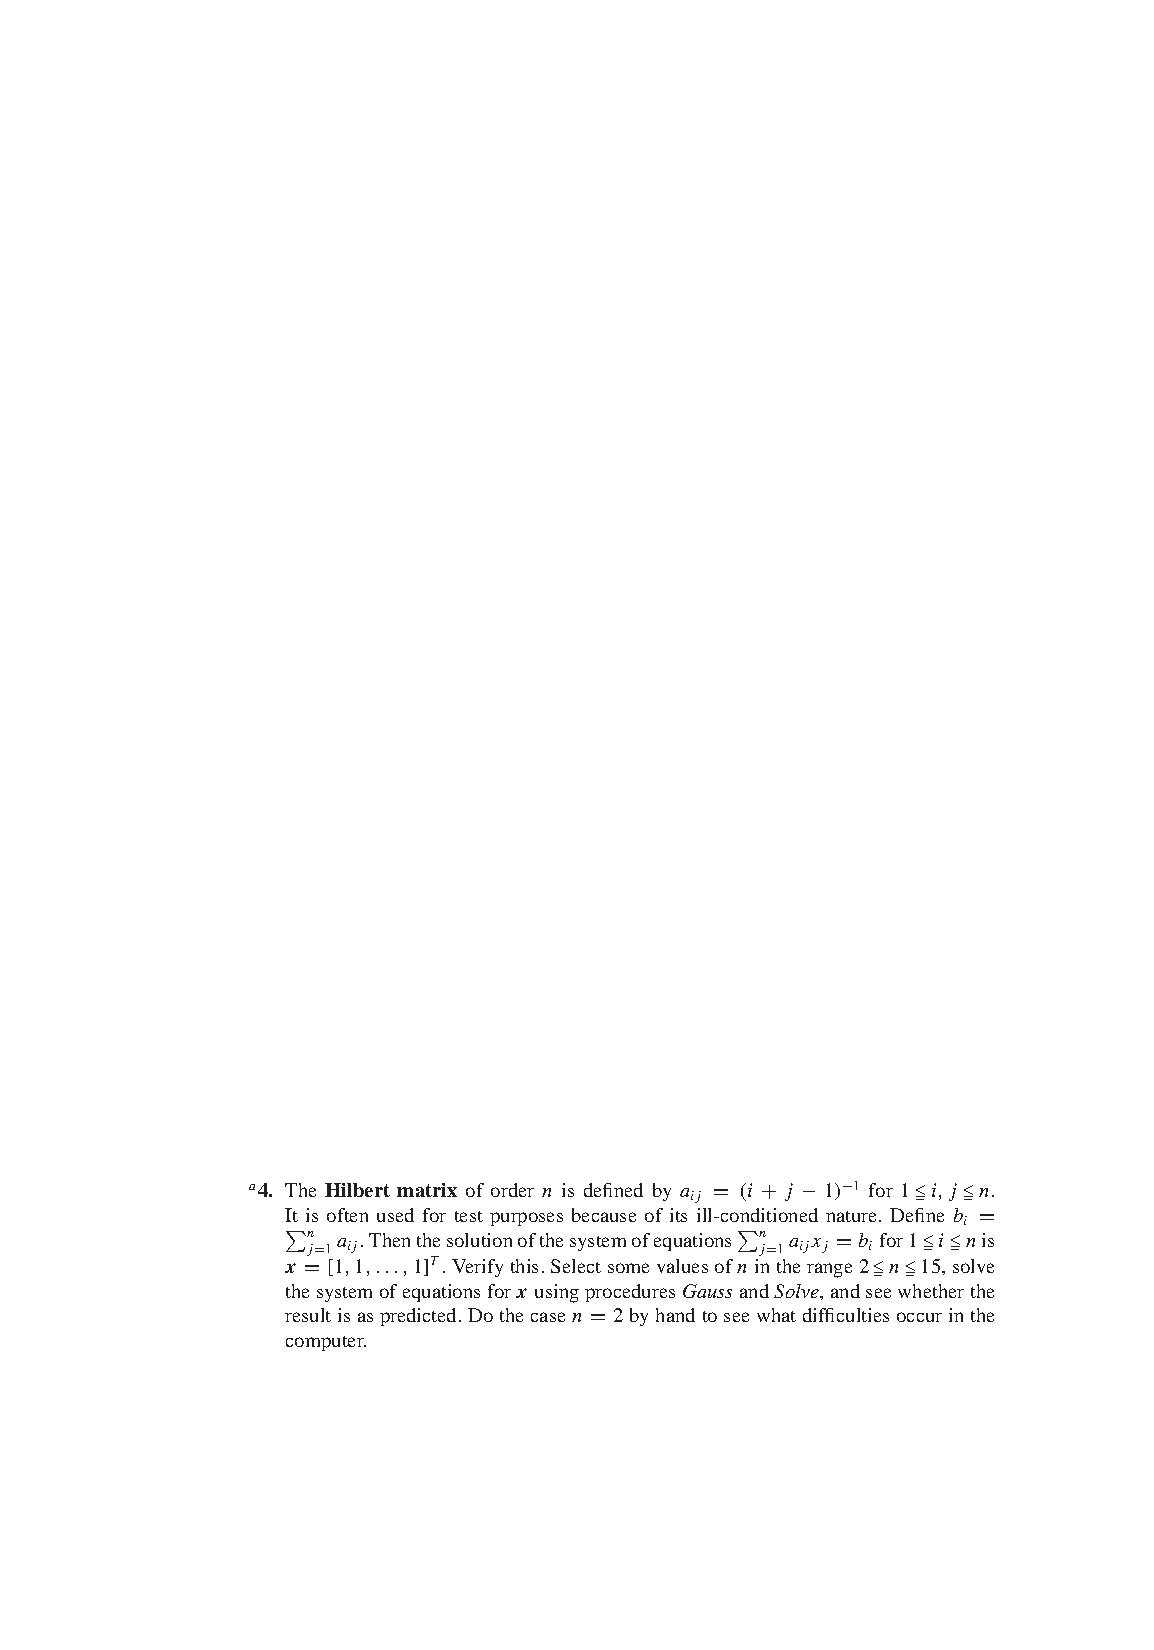
\includegraphics[width=1.0\textwidth]{fig/problem-02.pdf}
\end{figure}
\vfill
\end{frame}

\section*{Acknowledgments}
\label{sec:org0960aa4}
\begin{frame}[standout,label=]{}
Thank you
\end{frame}

\section{Bibliography}
\label{sec:org9dfe073}
\bibliographystyle{unsrt}
\bibliography{biblio} 
\cite{*}
\end{document}